% !TeX TXS-program:compile = txs:///pdflatex/[--shell-escape]
\documentclass[11pt,a4paper]{exam}
\printanswers % pour imprimer les réponses (corrigé)
%\noprintanswers % Pour ne pas imprimer les réponses (énoncé)
\addpoints % Pour compter les points
\usepackage[utf8]{inputenc}
\usepackage{minted}

%\usepackage[margin=1 in]{geometry}
\usepackage[a4paper,top=2.5cm,bottom=2.5cm,left=1.5cm,right=1.5 cm,marginparwidth=1.75cm]{geometry}
\usepackage{amsmath,amssymb}
\usepackage{multicol}
\usepackage{graphicx}
\usepackage{setspace}
\usepackage{dashundergaps}
\usepackage{tabularx} % Pour les tableaux ajustables
\usepackage{xcolor} % pour utiliser \cellcolor
\usepackage{colortbl} % pour les cellules colorées
% Définit une nouvelle colonne centrée verticalement et horizontalement
\newcolumntype{Y}{>{\centering\arraybackslash}X}
\renewcommand\tabularxcolumn[1]{m{#1}} % Centrage vertical pour X et Y
% Pour les graphes (dans la correction)
\usepackage{tikz}
\usetikzlibrary{graphs,graphs.standard,positioning}

% Pour afficher des numéros de ligne dans verbatim
\usepackage{listings}
\lstset{
	basicstyle=\ttfamily, % Set the basic style to typewriter font
	numbers=left,         % Position line numbers on the left
	numberstyle=\tiny,    % Set the style of the line numbers
	stepnumber=1,         % Line number increment
	numbersep=5pt,        % How far the line numbers are from the code
	%frame=single,         % Adds a frame around the code
	tabsize=2,            % Sets default tabsize to 2 spaces
	breaklines=true,      % Enables line breaking
	breakatwhitespace=false, % Break lines not only at whitespaces
}


\newcommand{\examnum}{Contrôle majeur \#4}
\newcommand{\class}{SNT 2\textsuperscript{nde}}
\newcommand{\examdate}{26/05/2024}
\newcommand{\timelimit}{45 Minutes}
\newcommand{\lycee}{Lycée Fustel de Coulanges}

\pagestyle{head}
\firstpageheader{}{}{}
\runningheader{\class}{\examnum\ - Page \thepage\ / \numpages}{\examdate}
\runningheadrule


\begin{document}
% Espace d'en-tête
\noindent
\begin{spacing}{1,2}
	\noindent
	\begin{tabular*}{\textwidth}{l @{\extracolsep{\fill}} l @{\extracolsep{6pt}} l}
		\textbf{\class} & \textbf{\examnum, \examdate}&\\
		\textbf{\lycee} &\textbf{Durée: \timelimit} &\\
	\end{tabular*}\\
\end{spacing}

\noindent
\vspace{10pt}
\hrule
\vspace{5pt} 

\begin{spacing}{1,2}
\vspace{\baselineskip}
\noindent
Ce contrôle comporte \numquestions\ questions; le maximum possible de points est de \numpoints\ points.\\ 
Les réponses sont à porter sur une \uline{\textbf{copie}} (\textbf{PAS} un morceau de papier arraché d'un cahier ou une copie déchirée) \uline{comportant votre nom}.\\
Il n'est pas nécessaire de répondre aux questions dans l'ordre \textemdash\ commencez par celles où vous vous sentez le plus à l'aise (mais numérotez bien les questions sur votre copie).\\
Les calculatrices ne sont \uline{pas} autorisées.\\
\noindent
\hrule
\vspace{15pt} 


        \begin{questions} % DEBUT DE L'EXAMEN
        	
        	\question {\textit{QCM}} -- reportez sur votre copie la réponse correcte \textit{en mentionnant bien la lettre de la question}.
			\begin{parts}
				\part[1]Pour effectuer un positionnement GPS on a besoin de...
        			\begin{choices}
		        			\choice 2 satellites: un au nord, un au sud.
		        			\choice 4 satellites: deux pour la latitude, deux pour la longitude.
		        			\correctchoice 4 satellites: 3 pour la triangulation, un pour la synchronisation de l'horloge.
		        			\choice 6 satellites: deux pour chaque dimension.
        			\end{choices}
        		\part[1]Le signal envoyé par les satellites du réseau GPS...
	        		\begin{choices}
	        			\choice Contient la position du satellite.
	        			\correctchoice Contient la position du satellite ainsi que l'heure d'envoi.
	        			\choice Contient la position du satellite, l'heure d'envoi et la marque du GPS.
	        			\choice Ne contient rien: c'est juste un "ping".
	        		\end{choices}
        		\part[1]Qu'est-ce que la théorie des six degrés de séparation?
	        		\begin{choices}
	        			\correctchoice L'idée que toute personne au monde est liée à une autre en 6 étapes maximum.
	        			\choice Quelque chose qui se passe quand on envoie un mail à plus de 6 personnes.
	        			\choice L'idée qu'un groupe d'amis cesse de fonctionner au-delà de 6 membres.
	        			\choice Une théorie qui dit qu'il faut être sur 6 réseaux sociaux différents.
	        		\end{choices}
	        	\part[1]Qu'est-ce que le cyberharcèlement?
	        		\begin{choices}
	        			\choice Une insulte publiée sur internet.
	        			\choice Des publicités qui reviennent sans cesse sur internet.
	        			\choice C'est un concept fictif qui a été inventé dans un roman américain de 2014.
	        			\correctchoice Une forme de violence répétée sur internet.
	        		\end{choices}
	        		
			\end{parts}
			        	
        	\question{\textit{Calcul d'itinéraire}}
        	
        	Soit la table suivante (fictive bien entendu):
        	
        	\begin{tabularx}{\textwidth}{|c|Y|Y|Y|Y|}
        		\hline
        		\rowcolor{gray!50} % Applique un fond gris à la ligne des en-têtes
        		\textbf{Lieux} & \textbf{Massy} & \textbf{Versailles} & \textbf{Palaiseau} & \textbf{Orsay} \\
        		\hline
        		\textbf{Massy} & \cellcolor{gray!20} - & 15 km / 20 min & 4 km / 20 min & Pas de route directe \\
        		\hline
        		\textbf{Versailles} & 15 km / 20 min & \cellcolor{gray!20} - & 12 km / 18 min & 10 km / 16 min \\
        		\hline
        		\textbf{Palaiseau} & 4 km / 20 min & 12 km / 18 min & \cellcolor{gray!20} - & 5 km / 18 min \\
        		\hline
        		\textbf{Orsay} & Pas de route directe & 10 km / 16 min & 5 km / 18 min & \cellcolor{gray!20} - \\
        		\hline
        	\end{tabularx}
        	
        	\begin{parts}
        		\part[2] Représenter cette table sous la forme d'un graphe.
        		\begin{solution}
        			\begin{figure}[H]
        				\centering
        				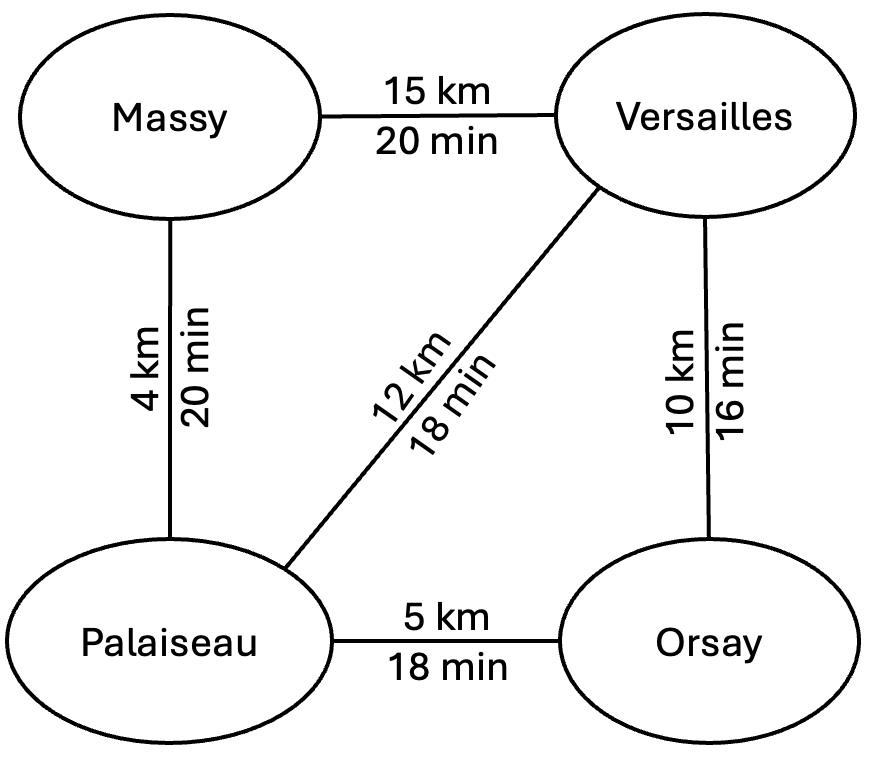
\includegraphics[width=0.4\textwidth]{GrapheVilles.png}
        			\end{figure}
        		\end{solution}
        		\part[1] Quel est le trajet le plus rapide entre Massy et Orsay?
        		\begin{solution}
        			Massy $\rightarrow$ Versailles $\rightarrow$ Orsay: 36 minutes.
        		\end{solution}
        		\part[1] Quel est le trajet le plus court en kilomètres entre Massy et Orsay?
        		\begin{solution}
        			Massy $\rightarrow$ Palaiseau $\rightarrow$ Orsay: 9 kilomètres.
        		\end{solution}
        	\end{parts}
        	
        	\question{\textit{Réseau social d'étudiants en informatique}}
        	
        	Soit le réseau social suivant constitué des personnes: Léa, Marc, Nina, Olivier, Pauline, et Quentin, avec les relations d'amitié suivantes:
        	\begin{itemize}
        		\item Léa est amie avec Nina.
        		\item Marc est ami avec Pauline.
        		\item Nina est amie avec Léa et Quentin.
        		\item Olivier est ami avec Pauline et Quentin.
        		\item Pauline est amie avec Marc, Olivier et Quentin.
        		\item Quentin est ami avec Nina, Olivier et Pauline.
        	\end{itemize}
        	
        	\begin{parts}
        		\part[2] Sur votre copie, écrivez le tableau d'adjacence pour représenter les relations d'amitié. On rappelle que les lignes et les colonnes seront constituées des noms des étudiants et que la diagonale ne comportera que des 0 (puisqu'on n'est pas ami avec soi-même).
        		\begin{solution}
        			\pagebreak
        			\[
        			\begin{array}{c|cccccc}
        				& \textbf{Léa} & \textbf{Marc} & \textbf{Nina} & \textbf{Olivier} & \textbf{Pauline} & \textbf{Quentin} \\
        				\hline
        				\textbf{Léa} & 0 & 0 & 1 & 0 & 0 & 0 \\
        				\textbf{Marc} & 0 & 0 & 0 & 0 & 1 & 0 \\
        				\textbf{Nina} & 1 & 0 & 0 & 0 & 0 & 1 \\
        				\textbf{Olivier} & 0 & 0 & 0 & 0 & 1 & 1 \\
        				\textbf{Pauline} & 0 & 1 & 0 & 1 & 0 & 1 \\
        				\textbf{Quentin} & 0 & 0 & 1 & 1 & 1 & 0 \\
        			\end{array}
        			\]
        		\end{solution}
        		\part[2] Représentez ce réseau sous forme de graphe.
        		\begin{solution}
        			\begin{figure}[H]
        				\centering
        				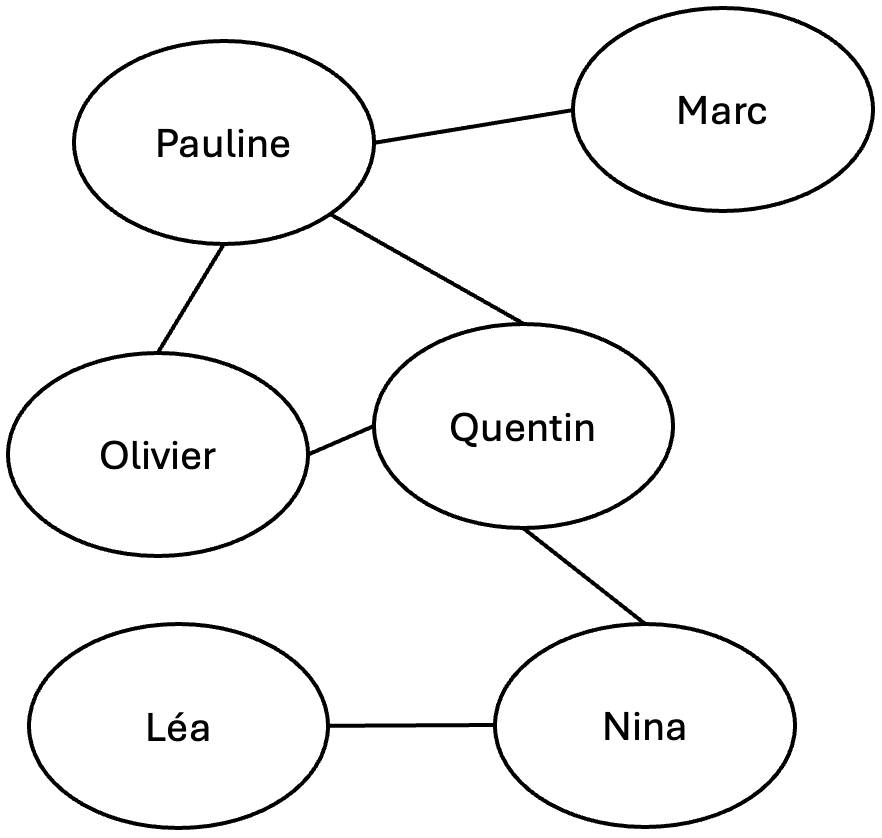
\includegraphics[width=0.4\textwidth]{GrapheResSoc.png}
        			\end{figure}
        		\end{solution}
        		\part Déterminez les distances entre les sommets suivants en spécifiant le chemin auxquelles elles correspondent:
        		\begin{subparts}
        			\subpart[1] Distance entre Léa et Olivier.
        			\begin{solution}
        				3 (Léa $\rightarrow$ Nina $\rightarrow$ Quentin $\rightarrow$ Olivier)
        			\end{solution}
        			\subpart[1] Distance entre Marc et Quentin.
        			\begin{solution}
        				2 (Marc $\rightarrow$ Pauline $\rightarrow$ Quentin)
        			\end{solution}
        		\end{subparts}
        		\part[2] Déterminez le centre du graphe (en incluant une phrase de justification de votre réponse).
        		\begin{solution}
        			Le centre d'un graphe est le (ou les, il peut y en avoir plusieurs) sommet du graphe dont la distance maximale à un autre sommet du graphe est la plus faible de tous les  sommets. Ce graphe compte \uline{\textbf{un seul centre, Quentin}}, dont la distance à tous les autres sommets ne dépasse jamais 2 (c'est le cas pour Léa et Marc). Tous les autres sommets du graphe ont au moins une distance de 3 par rapport à un des autres sommets:
        			\begin{itemize}
        				\item Léa $\leftrightarrow$ Marc = 4.
        				\item Nina $\leftrightarrow$ Marc = 3.
        				\item Pauline $\leftrightarrow$ Léa = 3.
        				\item Olivier $\leftrightarrow$ Léa = 3.
        			\end{itemize}
        		\end{solution}
        		\part[2] Déterminez le diamètre du graphe (en incluant une phrase de justification de votre réponse).
        		\begin{solution}
        			On rappelle que le diamètre d'un graphe est le plus long des plus courts chemins entre deux sommets du graphe. Dans ce cas, le diamètre est 4, car la distance maximale entre deux sommets est de 4 (Léa $\leftrightarrow$ Marc).
        		\end{solution}
        		
        	\end{parts}

			\question[3]{\textit{Leviers psychologiques utilisés par les médias sociaux}}
        	
        	À partir de l’épisode de la série Arte \uline{Dopamine} que vous avez vu en classe, identifiez et nommez un ressort psychologique spécifique utilisé par un média social que vous avez étudié (précisez lequel). Décrivez ce ressort et expliquez en au moins cinq phrases comment il est exploité par le média social pour encourager et maximiser l’engagement de ses utilisateurs.
        	\begin{solution}
        		Il y avait de multiples possibilités --- la validation sociale avec Instagram, les neurones miroir avec Tiktok, FOMO (\textit{Fear Of Missing Out}) ou l'escompte hyperbolique avec Twitter / X... Pour la correction je vous renvoie aux vidéos de la série. Ce qui importait dans la réponse soumise était:
        		\begin{itemize}
        			\item Nommer le ressort psychologique;
        			\item Clairement l'associer à un média social spécifique;
        			\item Fournir quelques éléments d'explication quant à son fonctionnement.
        		\end{itemize}
        	\end{solution}
        	
  
        \end{questions}
    \end{spacing}
\end{document}

% NON UTILISE:
\question[2]{\textit{Communication avec les satellites}}

\textit{On prendra dans cette exercice $300\text{ }000\text{ km.s}^{-1}$ comme approximation de la vitesse de la lumière.}
\begin{parts}
	\part[1] Vous recevez un signal d'un satellite. Ce message a été envoyé à 17 h 08 min 10,000 000 s, vous le recevez à 17 h 08 min 10,120 000 s. Déterminer la distance entre vous et le satellite.
	\part[2] Vous vous déplacez. Vous recevez un nouveau signal du satellite qui a mis 0,120 200 s pour vous atteindre. De combien de mètres vous êtes-vous déplacé\textperiodcentered e par rapport au satellite?
\end{parts}

\begin{solution}
	MCOXXXX
\end{solution}

%------------------------------------------
\question[2]{\textit{Réseau social d'étudiants en informatique}}

Considérons le réseau social des étudiants suivant :
\begin{itemize}
	\item Alice suit David, Emma et Hugo,
	\item Bruno suit Alice, Emma et Isabelle,
	\item Clara suit Alice et David,
	\item David suit Bruno et Clara,
	\item Emma suit Clara, Hugo et Isabelle,
	\item Hugo suit Bruno,
	\item Isabelle suit Alice et Emma.
\end{itemize}

\begin{parts}
	\part[1] Sur votre copie, écrivez le tableau d'adjacence pour représenter les relations de suivi entre ces étudiants. On rappelle que les lignes et les colonnes seront constituées des noms des étudiants, que la diagonale ne comportera que des 0 (puisqu'on ne se suit pas soi-même), et on utilisera le sens de lecture "ligne \textit{\textbf{suit}} colonne". Ainsi le coin haut gauche de la table d'adjacence aura cet aspect:
	\begin{figure}[H]
		\centering
		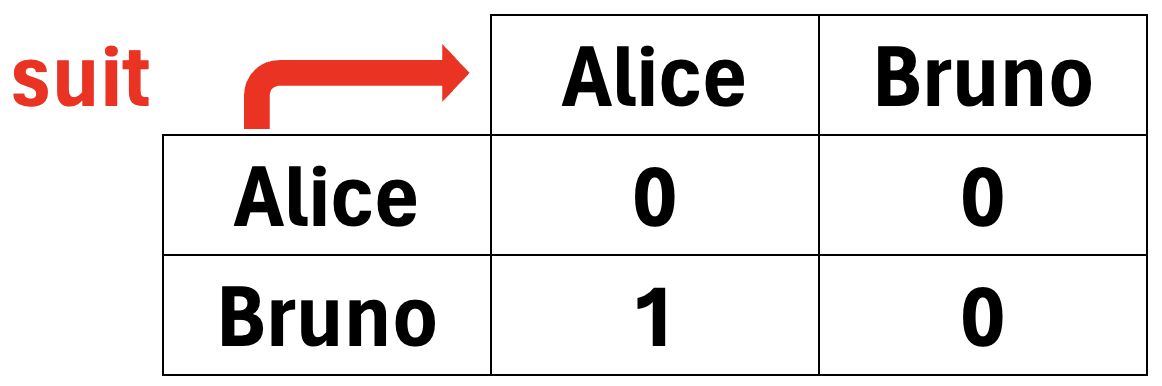
\includegraphics[width=0.3\textwidth]{TabAdj.png}
	\end{figure}
	\part[1] Comment peut-on déterminer le nombre de personnes qui suit Hugo?
	\part[1] Représenter ce réseau social sous forme d’un graphe.
	
\end{parts}

\begin{solution}
	MCOXXX
\end{solution}

% Graphe en latex - vraiment trop chiant versus screenshot dans PPT
        			\begin{tikzpicture}[node distance=2cm, every node/.style={circle, draw, minimum size=1.5cm}]
	\node (Marc) {Marc};
	\node[above right=of Marc] (Lea) {Léa};
	\node[below right=of Marc] (Nina) {Nina};
	\node[below left=of Nina] (Quentin) {Quentin};
	\node[below left=of Marc] (Pauline) {Pauline};
	\node[below=2cm of Quentin] (Olivier) {Olivier};
	
	\draw (Lea) -- (Nina);
	\draw (Nina) -- (Quentin);
	\draw (Pauline) -- (Quentin);
	\draw (Pauline) -- (Olivier);
	\draw (Quentin) -- (Olivier);
	\draw (Pauline) -- (Marc);
\end{tikzpicture}
